% !TeX spellcheck = pt_PT
%% ************************************************
%% Universidade Nova de Lisboa
%% NOVA Information Management School
%% Computação em Estatística e Gestão de Informação
%% Júlio Caineta, 2016
%% **********************************************
\documentclass{exam}
\usepackage[utf8]{inputenc}
\usepackage[portuguese]{babel}
\usepackage[hidelinks,pdfusetitle]{hyperref}
\author{Júlio Caineta}
\title{CEGI 2015/2016 - Exercícios 4}
\usepackage{lastpage}
\usepackage{minted}
\usepackage{paralist}
\usepackage{upquote}
\usepackage{amsmath}
\usepackage{graphicx}
%\usepackage{color}
\cfoot{Página \thepage\ de \pageref{LastPage}}
\renewcommand{\solutiontitle}{\noindent\textbf{Solução:}\par\noindent}
\newminted{r}{autogobble}
\newmintinline{r}{}
 
%\printanswers
%\shadedsolutions

\begin{document}
 
\begin{center}
\textsc {\small NOVA IMS -- Universidade Nova de Lisboa} \\
\textsc {Computação em Estatística e Gestão de Informação -- 2º Semestre 2015/16}
\vspace{5mm} \\
{\large Exercícios 4}
\end{center}
 
\vspace{5mm}

\section*{Manipulação de ficheiros e de dados}

Em termos computacionais, a informação é habitualmente transmitida em blocos a que denominamos ficheiros. O \textbf{R} disponibiliza uma vasta colecção de funções para manipular ficheiros de diferentes formatos. Neste exercício, pretende-se fazer uso de algumas funções de manipulação de ficheiros, e dos objectos resultantes do seu carregamento numa sessão de \textbf{R}.

Para treinar esses conceitos, considere o papel de um analista de dados desportivos. A sua tarefa é recolher, preparar e analisar um conjunto de dados da \textit{Primeira Liga} de futebol portuguesa (\autoref{fig:fcp}).

\begin{figure}[h]
	%\vspace{-40pt}
	\centering
	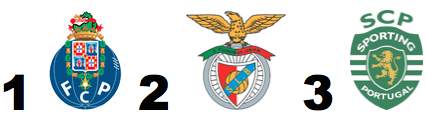
\includegraphics[width=0.4\linewidth]{fcp}
	%\vspace{-10pt}
	\caption{Preferências clubísticas à parte, eis o que os dados revelam.}
	\label{fig:fcp}
\end{figure}

Recorde algumas das funções que lhe poderão ser úteis na resolução deste tipo de problemas (use o sistema de ajuda para verificar como as usar):

\begin{description}
	\item[Operações matemáticas comuns] mean, sum, colMeans, rowMeans
	\item[Outros estatísticos] min, max, sd, var
	\item[Propriedades de objectos tabulares] nrow, ncol, names, colnames, rownames
	\item[Sumarizar e contar] summary, str, table, margin.table, which, which.max, which.min
	\item[Aplicar funções sobre objectos] apply, sapply, tapply
	\item[Ordenação] sort, order, rank
	\item[Agregação e manipulação] by, aggregate, transform
	\item[Manipular strings] substr, strsplit, paste, nchar
\end{description}

 
\begin{questions}
\question  Recolha os dados existentes na seguinte tabela das últimas 25 temporadas:

\begin{center}
	\url{http://www.european-football-statistics.co.uk/atc/atcprt.htm}
\end{center}

Esta tabela contém alguns dados sobre as 43 equipas que participaram nessas temporadas. Os dados estão agrupados nas seguintes variáveis:

\begin{description}
	\item[No.] Posição
	\item[Club] Nome da equipa
	\item[G] Jogos
	\item[W] Vitórias
	\item[D] Empates
	\item[L] Derrotas
	\item[P] Pontos
	\item[F] Golos marcados
	\item[A] Golos sofridos
	\item[S] Temporadas
	\item[1] Vencedor
	\item[2] Segundo lugar
	\item[3] Terceiro lugar
	\item[Cup] Taças de Portugal
\end{description}

Existem várias formas possíveis de recolher dados de uma página na \textit{World Wide Web}. Uma delas, usando o \textbf{R}, e para o caso de os dados estarem em forma de uma tabela, é através da função \rinline{readHTMLTable(url)}, que é disponibilizada no pacote (\textit{package}) XML.

\textbf{Nota:} O \textbf{R} já vem com alguns pacotes instalados. Pode instalar um novo pacote usando a função \rinline{install.packages('nome-do-pacote')}. Para importar o conteúdo de um pacote para a sessão actual, usa-se a função \rinline{library(nome-do-pacote)}. Repare que no primeiro caso o nome do pacote é passado como \rinline{character}, enquanto que no segundo caso não.

\begin{solution}
\begin{rcode}
	url = 'http://www.european-football-statistics.co.uk/atc/atcprt.htm'
	tabelas = readHTMLTable(url, stringsAsFactors=FALSE)
\end{rcode}
\end{solution}

\question Verifique a estrutura da operação anterior. Irá reparar que a função \rinline{readHTMLTable()} procura ler todas as tabelas existentes numa página, mesmo as que não sejam óbvias para o leitor, mas que sejam tabelas por definição (código HTML). Guarde a tabela de interesse numa variável chamada \rinline{liga}.

\begin{solution}
	Esta função devolve uma lista, tal como se pode verificar com a função \rinline{str()}.
	\begin{rcode}
		str(tabelas)
		liga = tabelas[[3]]
	\end{rcode}
\end{solution}

\question  Uma vez que os dados estejam importados, é necessário confirmar se estão no formato certo e que não há irregularidades.

Parece que a coluna 8 não é mais do que um artefacto na tabela. Remova-a da tabela.

\begin{solution}
	Basta escolher todas as colunas menos a que se pretende apagar.
	\begin{rcode}
		liga = liga[-8]
	\end{rcode}
	Alternativamente, também se pode igualar a coluna que se pretende apagar a \rinline{NULL}. Esta abordagem não funcionaria caso se tratasse de uma matriz e não de um data frame.
	\begin{rcode}
		liga[8] = NULL
	\end{rcode}
\end{solution}

\question Verifique o tipo de dados em cada uma das colunas. Corrija as colunas que não estiverem no formato mais adequado (por exemplo, uma coluna numérica estar no formato de texto).

\begin{solution}
	Solução dada em conjunto com o exercício seguinte.
	
	\textbf{Nota:} No caso de resolver este exercício em separado do exercício 5, dependendo de como resolver, é possível que alguns números sejam importados de forma errada (e.g., 1.908 em vez de 1908). Assim, sugere-se que resolva os dois em simultâneo, como nesta resolução, ou primeiro o 5 e depois o 4.
\end{solution}

\question Frequentemente, os dados incluem erros ou inconsistências na sua formatação. Esta tabela é mais um exemplo disso. Essas incongruências têm que ser tratadas antes de se proceder à análise de dados. Repare nas colunas \textbf{F}, \textbf{A} e \textbf{P}. Qual o problema que identifica?

Depois de ter identificado o problema, reconhecerá a utilidade do seguinte exemplo para o resolver.

\begin{rcode}
	> x = c("aaa", "bb.b", "cc,c")
	> x = gsub("\\.", "", x)
\end{rcode}

\textbf{Nota:} É possível resolver este exercício e o anterior numa só vez.

\begin{solution}
	A maior parte dos números (mas não todos!) usa o ponto como separador dos milhares. É necessário remover o ponto, para que os números sejam correctamente identificados em \textbf{R}, caso contrário, poderão vir a ser reconhecidos como números decimais. A segunda coluna é a única que deverá manter-se como texto, pois contém o nome dos clubes.
	\begin{rcode}
		str(liga)
		liga[-2] = apply(liga[-2], 2, function(coluna) as.numeric(gsub("\\.", "", coluna)))
	\end{rcode}
\end{solution}

\question Concluída a preparação dos dados, há que passar à análise. Quais são as equipas com mais derrotas do que a média?

\begin{solution}
	\begin{rcode}
		subset(liga, L > mean(L))
	\end{rcode}
\end{solution}

\question Acrescente uma nova coluna com a média de golos por jogo de cada equipa.

\begin{solution}
	\begin{rcode}
		liga = transform(liga, média_golos = F / G)
	\end{rcode}
\end{solution}

\question Como acrescentou uma coluna ao conjunto de dados, já vale a pena guardar os dados num ficheiro. Guarde-os num novo ficheiro com a seguinte especificação:

\begin{description}
	\item[Nome] PrimeiraLiga\_25anos.dat
	\item[Separador] tabulação
	\item[Separador decimal] vírgula
	\item[Valores em falta (\rinline{NA})] hífen
	\item[Nome das colunas] sim
	\item[Nome das linhas] não
\end{description}

\begin{solution}
	\begin{rcode}
		nome = 'Primeira_Liga_25anos.data'
		write.table(file=nome, sep='\t', dec=',', na='-', col.names=TRUE, row.names=FALSE)
	\end{rcode}
\end{solution}

\question Nem sempre um maior número de pontos corresponde a um maior número de vitórias. Identifique as equipas em que a sua posição na tabela (está ordenada por pontos) não corresponde à posição se a tabela estivesse ordenada por vitórias.

\begin{solution}
	\begin{rcode}
		liga$Club[order(liga$W, decreasing=TRUE) != liga$No.]
	\end{rcode}
	%$
\end{solution}

\question Qual é a equipa que tem mais golos marcados do que sofridos, e que simultaneamente tem menos pontos?

\textbf{Sugestão:} Acrescente primeiro uma coluna que diz se a equipa tem ou não mais golos marcados do que sofridos.

\begin{solution}
	\begin{rcode}
		liga = transform(liga, positivo = F - A > 0)
		liga$Club[max(which(liga$positivo))]
	\end{rcode}
\end{solution}

\question Haverá uma relação entre o número de golos e o número de temporadas, isto é, se, em média, as equipas com mais experiência na \textit{Primeira Liga} tendem a marcar mais golos?

\textbf{Sugestão:} Determine primeiro qual a média de golos marcados por cada valor de experiência (número de épocas jogadas).

\begin{solution}
	\begin{rcode}
		média_época = aggregate(liga$G, list(liga$S), mean)
		média_época = transform(média_época, média = x / Group.1)
		> média_época
		Group.1         x        m
		1        1  32.00000 32.00000
		2        2  66.00000 33.00000
		3        3  99.71429 33.23810
		4        4 136.00000 34.00000
		5        5 163.33333 32.66667
		6        6 192.00000 32.00000
		7        7 238.00000 34.00000
		8        8 264.00000 33.00000
		9       11 374.00000 34.00000
		10      13 430.00000 33.07692
		11      14 452.00000 32.28571
		12      15 486.00000 32.40000
		13      16 518.00000 32.37500
		14      17 566.00000 33.29412
		15      18 651.00000 36.16667
		16      19 638.00000 33.57895
		17      20 654.00000 32.70000
		18      24 788.00000 32.83333
		19      25 818.00000 32.72000
	\end{rcode}
	Olhando para os valores, não parece haver uma relação entre o número de épocas jogadas e a média de golos marcados.
	
	Este facto pode ser confirmado com uma regressão linear (esta parte não era pedida no exercício, nem faz parte da matéria da disciplina, mas poderá ser útil aos alunos no futuro).
	
	\begin{rcode}
		coef(lm(média_época$m ~ média_época$Group.1))
		        (Intercept) média_época$Group.1
		        32.95632059          0.01388322
	\end{rcode}
	%$
	Essas duas variáveis têm um coeficiente de correlação muito baixo, cerca de 1,4\%.
	
\end{solution}

\question Normalmente os clubes são mais conhecidos por uma só palavra. Por exemplo, o clube \textit{SC de Braga} é conhecida por \textit{Braga}, e o clube \textit{A Naval 1º de Maio} é mais conhecido apenas por \textit{Naval}.

Pretende-se alterar o nome dos clubes  para a denominação mais comum. De modo a não alterar um a um manualmente, considere o seguinte algoritmo (não é perfeito, mas funciona bem na maior parte dos casos):

\begin{enumerate}
	\item Separar o nome por palavras;
	\item Escolher a palavra com maior número de caracteres;
	\item Usar essa palavra como nome para a equipa.
\end{enumerate}

Por exemplo, o clube com o nome \rinline{"CF Os Belenenses"} pode ser separado num vector com 3 palavras:

\begin{rcode}
	[1] "CF"         "Os"         "Belenenses"
\end{rcode}

Estas palavras têm os seguintes números de caracteres:

\begin{rcode}
	[1]  2  2 10
\end{rcode}

Neste vector, o valor mais alto está na posição:

\begin{rcode}
	[1] 3
\end{rcode}

Então, voltando ao vector com as palavras separadas, escolhe-se a palavra nessa posição:

\begin{rcode}
	[1] "Belenenses"
\end{rcode}	

\textbf{Nota:} Neste exercício, há uma função que pode ser particularmente útil, caso utilize listas como um resultado intermediário: \rinline{unlist()}. Esta função simplifica uma lista para a forma de um vector.

\begin{solution}
	\begin{rcode}
		palavra_mais_longa = function(nome) {
			palavras = unlist(strsplit(nome, " "))
			mais_longa = which.max(nchar(palavras))
			return (palavras[mais_longa])
		}
		
		sapply(liga$Club, palavra_mais_longa)
		
		             FC Porto            SL Benfica           Sporting CP
		             "Porto"             "Benfica"            "Sporting"
		             SC de Braga  Vitória SC Guimarães   CS Marítimo Madeira
		             "Braga"           "Guimarães"            "Marítimo"
		             Boavista FC      CF Os Belenenses  FC Paços de Ferreira
		             "Boavista"          "Belenenses"            "Ferreira"
		             Vitória FC Setúbal          UD de Leiria        Gil Vicente FC
		             "Vitória"              "Leiria"             "Vicente"
		             CD Nacional Madeira            Rio Ave FC   A Académica Coimbra
		             "Nacional"                 "Rio"           "Académica"
		             SC Beira Mar CF Estrela da Amadora            SC Farense
		             "Beira"             "Estrela"             "Farense"
		             SC Salgueiros 08      GD Estoril Praia          GD de Chaves
		             "Salgueiros"             "Estoril"              "Chaves"
		             Moreirense FC    A Naval 1º de Maio         FC de Alverca
		             "Moreirense"               "Naval"             "Alverca"
		             SC Campomaiorense          SC Olhanense   CF União da Madeira
		             "Campomaiorense"           "Olhanense"             "Madeira"
		             FC de Tirsense             FC Arouca           FC Penafiel
		             "Tirsense"              "Arouca"            "Penafiel"
		             Leça FC          FC Famalicão        CD Santa Clara
		             "Leça"           "Famalicão"               "Santa"
		             Varzim SC            Leixões SC         SC de Espinho
		             "Varzim"             "Leixões"             "Espinho"
		             CD Aves         SCU Torreense         FC Felgueiras
		             "Aves"           "Torreense"          "Felgueiras"
		             CD Tondela       Portimonense SC           CD Feirense
		             "Tondela"        "Portimonense"            "Feirense"
		             CD Trofense
		             "Trofense"
	\end{rcode}
	% $
\end{solution}

\end{questions}

\end{document}